\documentclass[12pt]{article}

\usepackage[T1]{fontenc}
\usepackage{mathptmx}

\topmargin 0.0in
\setlength{\textwidth} {420pt}
\setlength{\textheight} {620pt} 
\setlength{\oddsidemargin} {20pt}
\setlength{\marginparwidth} {72in}

\usepackage{fancyhdr} 
\usepackage{url}

% set it so that subsubsections have numbers and they
% are displayed in the TOC (maybe hard to read, might want to disable)

\setcounter{secnumdepth}{3}
\setcounter{tocdepth}{3}

% define widow protection

\def\widow#1{\vskip #1\vbadness10000\penalty-200\vskip-#1}

\clubpenalty=10000  % Don't allow orphans
\widowpenalty=10000 % Don't allow widows

% this should give me the ability to use some math symbols that 
% were available by default in standard latex (i.e. \Box)

\usepackage{latexsym}
\usepackage{graphicx}

% define a little section heading that doesn't go with any number

\def\littlesection#1{
\widow{2cm}
\vskip 0.5cm
\noindent{\bf #1}
\vskip 0.0001cm 
}

\pagestyle{fancyplain}

\newcommand{\tstamp}{\today}   
\renewcommand{\sectionmark}[1]{\markright{#1}}
\lhead[\Section \thesection]            {\fancyplain{}{\rightmark}}
\chead[\fancyplain{}{}]                 {\fancyplain{}{}}
\rhead[\fancyplain{}{\rightmark}]       {\fancyplain{}{\thepage}}
\cfoot[\fancyplain{\thepage}{}]         {\fancyplain{\thepage}{}}

\newlength{\myVSpace}% the height of the box
\setlength{\myVSpace}{1ex}% the default, 
\newcommand\xstrut{\raisebox{-.5\myVSpace}% symmetric behaviour, 
  {\rule{0pt}{\myVSpace}}%
}

% leave things with no spacing extra spacing in the final version of the paper
\renewcommand{\baselinestretch}{1.0}    % must go before the begin of doc

% suppress the use of indentation for a paragraph

\setlength{\parindent}{0.0in}
\setlength{\parskip}{0.1in}

\begin{document}

%% \begin{abstract}

%%   Try

%% \end{abstract}

% handle widows appropriately
\def\widow#1{\vskip #1\vbadness10000\penalty-200\vskip-#1}

% build the title section

\makeatletter

\def\maketitle{%
  %\null
  \thispagestyle{empty}%
  %\vfill
  \begin{center}%\leavevmode
    %\normalfont
% define a little s
    {\Huge \@title\par}%
    %\hrulefill\par
    \vspace*{.4in}
    {\normalsize \@author\par}%
    \vskip .5in
%    {\Large \@date\par}%
  \end{center}%
  %\vfill
  %\null
  %\cleardoublepage

  }

\makeatother

\vspace*{-1.1in}
\title{JDepend and JavaNCSS description Document}
\vspace*{-.1in}
% build the author section
\author{Adam Wechter, Matt Hajduk, Brian Graham, Shane Regel, Andreas Landgrebe\\
Department of Computer Science\\
Allegheny College \\
\vspace*{.4in} \today \\ \vspace*{.6in}
{\bf Abstract} \\ A description of the design metrics for JavaNCSS and JDepend. Also an analysis for each on the three systems implemented by our team.}

% use the default title stuff
\maketitle

\vspace*{.1in}
\section{JDepend}
\label{sec:JDepend}
\vspace*{-.1in}


\subsection{Description}

JDepend provides insight into several qualities of software architecture. JDepend analyzes the relationships between Java packages using class files. JDepend searches through file directories and generates design quality metrics for each Java package. It allows for the measurement of the quality of design in terms of its extensibility, reusability, and maintainability to manage package dependencies effectively. As described in Figure~\ref{figure1} two packages A and B are cyclically dependent if package A depends on package B, and package B depends on package A. This is referred to as a direct cycle. Cyclic dependencies impact the ability of developers to make changes to the system. Package Z and package A form what is called an indirect cyclic dependency. Package Z doesn't directly participate in a direct cycle, but because it depends on one (or more) packages that do participate in a direct cyclic relationship, it is inherently less stable. In the case of a dependency a simple change to a component of the system may affect a seemingly unrelated component.\\

\begin{figure}
\center
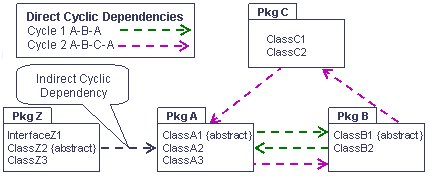
\includegraphics[width=.6\textwidth]{figure2.jpg} 
\caption{Dependency Cycles}
\label{figure1}
\end{figure}

\textbf{Number of Classes and Interface}\\
The number of concrete and abstract classes (and interfaces) in the package is an indicator of the extensibility of the package.\\ \\

\textbf{Afferent Couplings (Ca)}\\
The number of other packages that depend upon classes within the package is an indicator of the package's responsibility.\\ \\

\textbf{Efferent Couplings (Ce)}\\
The number of other packages that the classes in the package depend upon is an indicator of the package's independence.\\ \\

\textbf{Abstractness (A)}\\
The ratio of the number of abstract classes (and interfaces) in the analyzed package to the total number of classes in the analyzed package. The range for this metric is 0 to 1, with A=0 indicating a completely concrete package and A=1 indicating a completely abstract package.\\ \\

\textbf{Instability (I)}\\
The ratio of efferent coupling (Ce) to total coupling (Ce + Ca) such that 
\begin{equation}
I = \frac{Ce}{(Ce + Ca)}
\end{equation}
This metric is an indicator of the package's resilience to change. The range for this metric is 0 to 1, with I=0 indicating a completely stable package and I=1 indicating a completely instable package.\\ \\

\textbf{Distance from the Main Sequence (D)}\\
The perpendicular distance of a package from the idealized line A + I = 1. This metric is an indicator of the package's balance between abstractness and stability. A package squarely on the main sequence is optimally balanced with respect to its abstractness and stability. Ideal packages are either completely abstract and stable (x=0, y=1) or completely concrete and instable (x=1, y=0). The range for this metric is 0 to 1, with D=0 indicating a package that is coincident with the main sequence and D=1 indicating a package that is as far from the main sequence as possible.\\ \\

\textbf{Package Dependency Cycles}\\
Package dependency cycles are reported along with the hierarchical paths of packages participating in package dependency cycles.\\ \\

\subsection{Analysis}

\textbf{Lab 3 Analysis}\\
When observing the JDepend report on the packages and dependencies within the packages, we have a total of 2 Efferent Couplings and a package with an Instability of 1.  The instability level was determined by the following equation:
\begin{equation}
I = \frac{CA}{CA+CE}
\end{equation}
Since we have two efferent couplings and no afferent ones that means we have an incredibly high instability.  That means that it’s resilience to change is absent because of the lack of independent classes.  This is good though because we have a very low sense of abstractness meaning this will not be used in any other way other than implemented.  Additionally, since this is such a simple program, we actually have no abstract classes and the distance from the main sequence is at 0, meaning it coincides with the main sequence.  Finally we have 0 package dependency cycles which is a positive aspect to the integrity of the program.\\

\textbf{Lab 4 Analysis}\\
Listerino had a similar report to the first one with two efferent couplings and a high instability rating of 1.  This was after excluding the Junit classes since they do not have a direct effect on the actual project we are working on.  We had 5 concrete classes including the test classes and two \textit{depends upon} which were the two Junit packages, both org.junit and org.junit.runners.  once again this was a relatively good package since we had 0 package dependency cycles.  Once again, we see a very high instability rating which is not necessarily a bad thing because, again, our abstractness is a 0. \\

\textbf{Open Source - JDepend}\\
Jdepend was our choice of open source and it was a significantly larger than our previous analyzed projects.  There were a total of four packages examined and all of them had varying statistics.  The first is the framework under JDepend and has a total of 34 classes, 31 of which were concrete and 4 abstract classes, meaning extensible classes.  Out of these, there were a total of 3 afferent classes, and 13 efferent classes, leading to an Instability level of 0.81.  Additionally it has an abstractness level of .11 which is merely a representation of the proportion of abstract classes, as well as a distance from main sequence of 0.07.  This final measurement indicates that it coincides rather closely with the main sequence of this program.  The list of \textit{depends upon} can be found in the actual list which is delivered, and this package gets used by all 3 other packages measured in this report.  This is a change from the other packages since only other dependency package is the jdepend.textui package, which is used by xml which makes sense due to the nature of the xmlui.   \\


\vspace*{.1in}
\section{JavaNCSS}
\label{sec:JavaNCSS}
\vspace*{-.1in}

JavaNCSS is a source measurement suite for Java. Its a command line utility that measures two standard source code metrics in Java. The two metrics are collected for each class and function in the program. JavaNCSS looks at the number of Non Commenting Source Statements(NCSS), the Cyclomatic Complexity Number(CCN), and the number of Javadoc comments per class and method. 

The Non Commenting Source Statements gives the number of statements and declarations in the source files. Some examples that increment the counter of NCSS are package declarations, import declarations, method declarations, constructor declarations, interface declarations, etc. NCSS is technically equivalent to counting the semi colon and open bracket characters in the source files. 

The Cyclomatic Complexity Number shows how complex a program is by measuring the number of linearly independent paths in the source code. Simply, it is the number of if, for, while, case, catch,etc. statements in the source code. If the code has no if statements or for loops, then the code would have a Cyclomatic Complexity would be one because it has one linearly independent path. The Cyclomatic Complexity can be defined using a control flow graph of a program. The control flow graph is a directed graph with basic block nodes of the program and edges connecting the nodes. The complexity M is defined as: $M = E-N+2P$ where E is the number of edges in the graph, N is the number of nodes in the graph, and P is number of exit nodes in the graph. 


\subsection{Analysis}


Team four decided to use the lab three system, the lab four system, and the JDepend system, found on the JDepend website. This report will analyze the all three implementations of JavaNCSS on the three systems and the results that were calculated. The first system that will be discussed is lab four. The lab four system takes in an input list and uses a data generator to produce all of the lists that can be obtained by swapping two adjacent items in the list. The results above show the Non Commenting Source Statements(NCSS), Cyclomatic Complexity Number(CCN), and the number of Javadoc comments in the entire system, in each class, and each method. It shows that there is one package, four classes, and 30 functions(methods) in the entire system. It also shows there are 278 NCSS and 15 Javadoc comments throughout the system. The results show the The JavaNCSS also calculates the average NCSS, functions, inner classes, and Javadoc comments in each class. The lab four results for the average NCSS is 65.75 per class, 7.50 functions per class, 0 inner classes per classes, and 3.75 Javadoc comments per class. The JavaNCSS also looks at the CCN value of each function. The function with the highest CCN is the viewListArr(Object) found in the listerino class. The CCN of the function is seven because there are multiple declarations followed by one if statement and 3 for loops. The function that has the most NCSS in the system was main(String[]) found in the driver class. The function has 38 NCSS because there are a large amount of print statements.

The next system that team four implemented JavaNCSS in was the lab three system. Lab three was an introduction to eclim and used simple commands to find a defect in the kentic.java file. Just like the lab four results, the results from lab three show that the system is not very large or complex. If has one package with four classes and 13 functions(methods). The system has a total of 73 NCSS and 16 Javadoc comments. The JavaNCSS results also calculate the averages and values of the NCSS, functions, inner classes, and Javadoc comments for the classes and functions.  The function with the highest CCN in the lab three system was computeVelocity(int,int) . The computeVelocity method has the highest CCN because it has two declarations and an if statement to have a CCN of 3. The number of NCSS also correlates to the CNN because the more complex the function is the more NCSS it contains. For example, the computeVelocity function has a NCSS of 11, the most in the system.

The final system team four implemented JavaNCSS into was the JDepend system found on the JDepend website. The results showed that this system is more complex and very large compared to the other two systems the team looked at. The JDepend system consists of five packages with a total of 22 class and 275 functions throughout. The system is a very complex system and the function with the highest CCN is jjMoveNfa0(int,int). This function has a CCN of 230 and also has the highest NCSS of 496. The average CCN of each function is a 9.26 which shows that JDepend is a very complex system that has many paths through each function. 

\bibliographystyle{plain}
\bibliography{bibliography.bib}

\end{document}


